\subsection{Falling Sphere}
\label{sec:falling_sphere}

The conveyor belt case from the previous section favors the Lagged model due to
the steady-state normal force, where the Lagged model is exact. Here, we
introduce a collision test to evaluate approximations under sudden contact
force changes.

In this test, a $0.5\text{ kg}$ steel sphere $5\text{ cm}$ in diameter falls
from a height of $5\text{ cm}$ with an initial horizontal velocity $U_0=2\text{
m/s}$, see Fig. \ref{fig:sphere_schematic}. Friction with the ground is
$\mu=0.5$. Upon impact, the sphere slides, and then transitions to rolling
as friction induces angular momentum. After this transition, friction ceases to
dissipate energy. We model compliant contact with stiffness $k=10^{7}\text{
N/m}$ and dissipation constants $d=500\text{ s/m}$ and
$\tau_d=10^{-3}\text{ s}$.

\begin{figure}[!h]
    \centering
    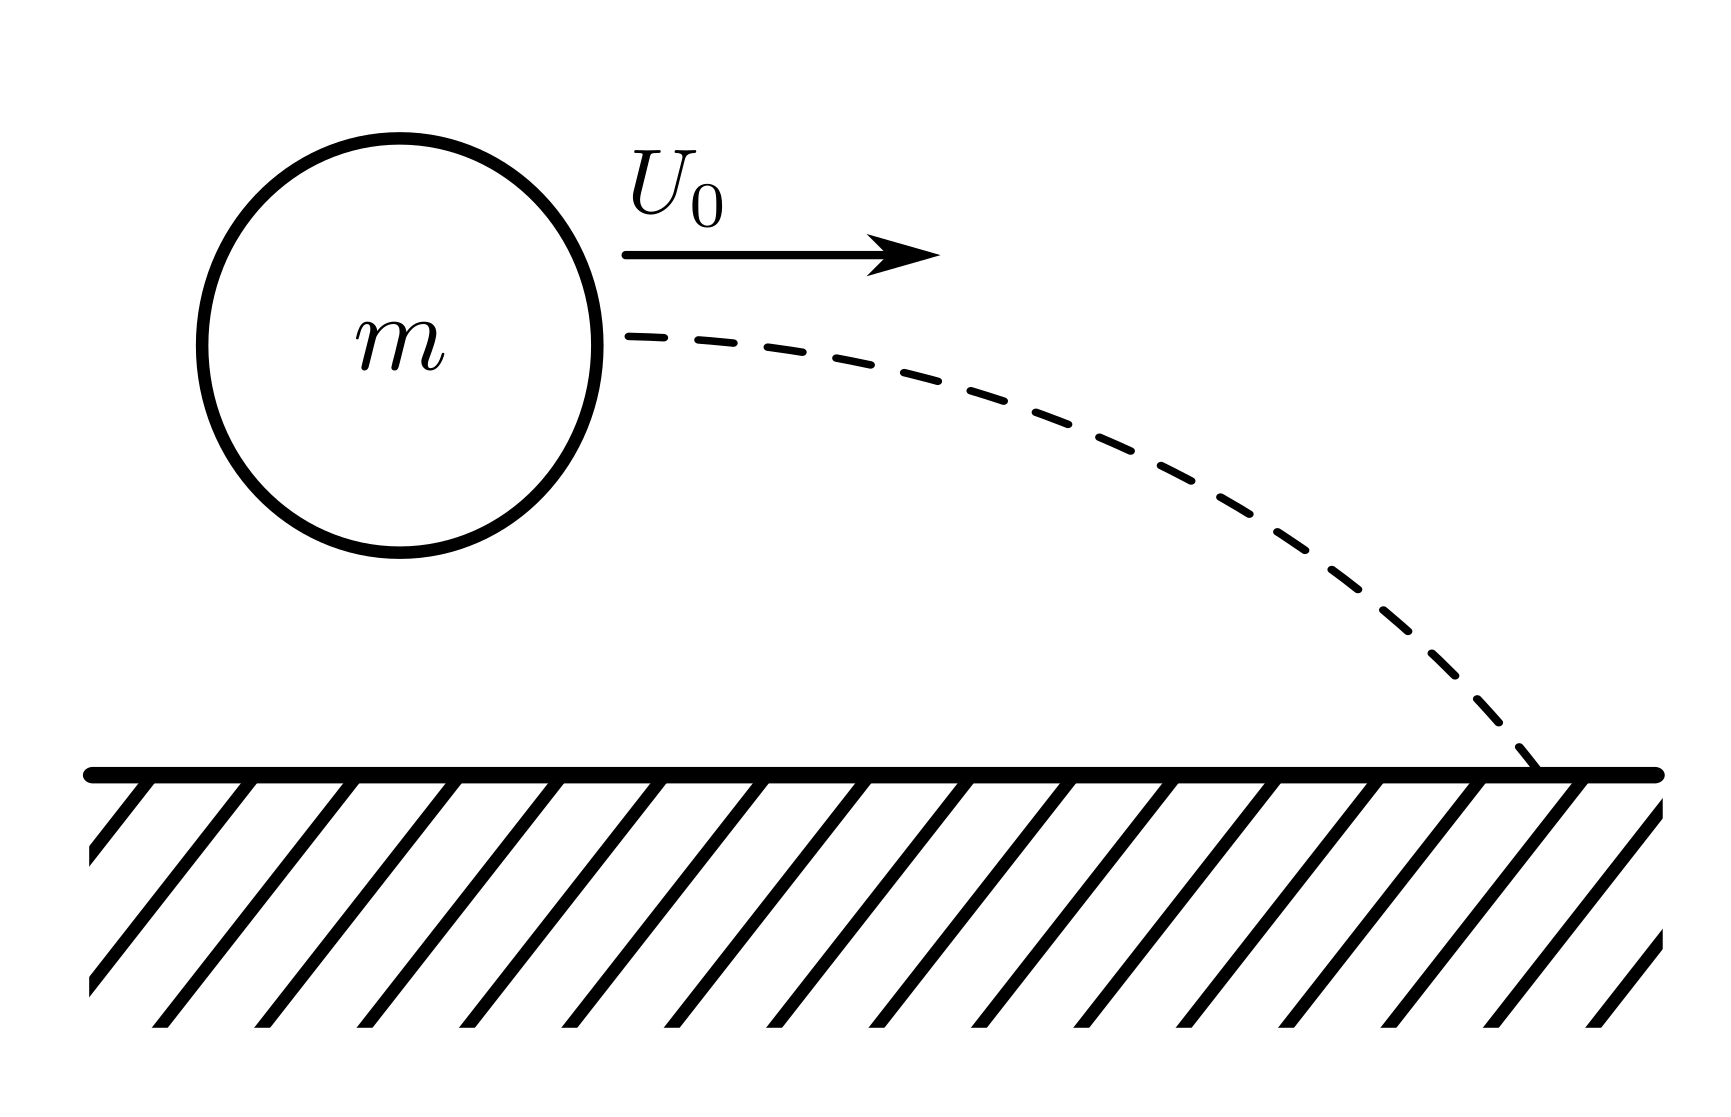
\includegraphics[width=0.6\columnwidth]{figures/TestCases/Cylinder/sphere_schematic.png}
    \caption{Falling sphere. After free fall, the sphere slides until friction with the ground establishes a rolling contact.}
    \label{fig:sphere_schematic}
\end{figure}

Figure \ref{fig:cylinder_contact_velocity_and_force} shows contact velocity and
force computed with $\delta t=2\times10^{-3}\text{ s}$. In the force plots, both
SAP and Similar initiate contact earlier due to the \emph{action at a distance}
artifact in these convex models, with SAP engaging even earlier due to the
non-vanishing term $\tau_d\mu\Vert\vf{v}_t\Vert$ in
\eqref{eq:sap_gliding_offset}. The sphere slides from initial contact until
about $t=0.07\text{ s}$, when it transitions to rolling. While Lagged brings
normal velocity to zero almost instantly, SAP and Similar models link normal
velocity to slip velocity, only reaching zero at stiction. During the
sliding-to-stiction transition, we observe a rapid normal force spike, as with
the conveyor belt problem. This artifact is absent with the Lagged
approximation.

\begin{figure}[!h]
    \centering
    %trim={<left> <lower> <right> <upper>}
    \adjincludegraphics[height=0.38\columnwidth,trim={0 0 {0.05\width} 0},clip]{figures/TestCases/Cylinder/contact_velocity_dt2em3.png}
    \adjincludegraphics[height=0.38\columnwidth,trim={0 0 {0.05\width} 0},clip]{figures/TestCases/Cylinder/contact_force_dt2em3.png}
    \caption{\label{fig:cylinder_contact_velocity_and_force} Contact velocity (left)
    and force (right) with $\delta t=2\times10^{-3}\text{ s}$.}
\end{figure}

A convergence study with step sizes $\delta t \in \{4\times10^{-4},
2\times10^{-3}, 10^{-2}\}$ is shown in Fig.
\ref{fig:cylinder_convergence_position}. While all of these schemes are first
order, SAP exhibits a constant error at convergence due to the
$\tau_d\mu\Vert\vf{v}_t\Vert$ term in \eqref{eq:sap_gliding_offset}.

\begin{figure}[!h]
    \centering
    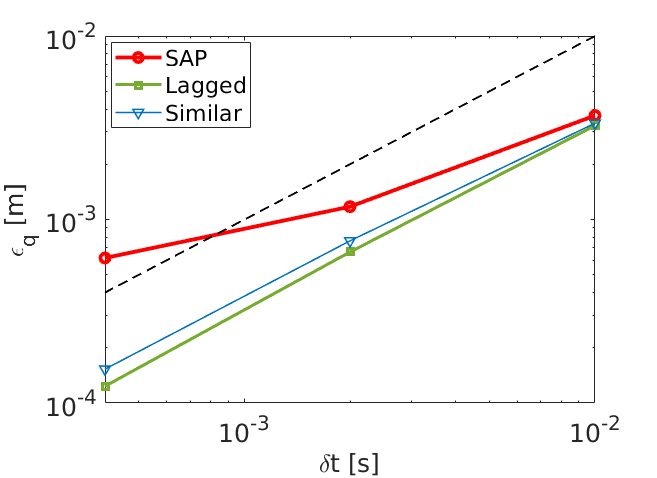
\includegraphics[width=0.8\columnwidth]{figures/TestCases/Cylinder/position_convergence.png}
    \caption{Convergence of the sphere trajectory with time step size. The dashed line is a reference for first order convergence.}
    \label{fig:cylinder_convergence_position}
\end{figure}
